\chapter{Review of literature and Model Selection } % Main chapter title

\label{Chapter3} % For referencing the chapter elsewhere, use \ref{Chapter2} 

Using content-based music information for solving several music information retrieval tasks is not new, but a decade long research efforts have been put. Hunting for the right model for our task and to justify it to be superior to the rest requires thorough understanding of evolution of such techniques. In section 3.1, the dynamics of the literature that has lead to the use of deep learning techniques for MIR tasks have been discussed. In section 3.2, the inferences from state of art techniques have been used to short list models for the experiments.       


\section{Evolution of algorithms}
A number of surveys (e.g. [8, 22, 29]) amply document what is a decades-long research effort at the intersection of music, machine learning and signal processing. In a broader sense, all techniques have a two-stage architecture: first, features are extracted from music audio signals to transform them into a more meaningful representation. These features are then used as input to a classifier, which is trained to perform the task at hand. This dedicated analysis for music features emerged due to the fact that music signals possess specific acoustic and structural characteristics that distinguish them from spoken language or other non musical signals. The motivation for writing this section elaborately is to make the answers for following questions clear,
\begin{enumerate}[label=(\alph*)]
\setlength\itemsep{0em}
\item To approach the solution, should we look for better classifier or better feature extractor?  
\item Can neural networks outperform features extracted through \gls{basis transformation} approaches on a medium sized dataset. What is the trade off between the both?
\item If deep learning had to be used, does fine-tuning (transfer learning) work for multi-label classification task? Are there any pre-trained models already available?
\end{enumerate}

\subsection{From classifier to feature emphasis}
Looking back to our history before 2010, there is a clear trend in MIR of applying increasingly more powerful machine learning algorithms to the same feature representations to solve a given task. There are also ample surveys with evidence suggesting that appropriate feature representations significantly reduce the need for complex semantic interpretation methods [2]. Evidence from genre classification and chord recognition task have been discussed below. 

\subsubsection{Audio music genre classification using different classifiers and feature selection methods. Proceedings of the International Conference on Pattern Recognition, Hong-Kong, China,2006}
Fixing the features, ten different classifiers were compared, namely: Fisher (Fisher classifier), LDC (Linear classifier assuming normal densities with equal covariance matrices), QDC (Quadratic classifier assuming normal densities), UDC (Quadratic classifier assuming normal uncorrelated densities), NBC (Naïve Bayes Classifier), PDC (Parzen Density Based Classifier), KNN (Knearest neighbor with optimal k computed using leave one out cross validation), KNN1 (1 nearest neighbor), KNN3 (3 nearest neighbor), KNN5.  It is seen that a ceiling performance of 80\% accuracy on GTZAN dataset was obtained by using combination of classifiers and squeezing every last percentage from the same features. This suggested the need for robust feature representation for further improvements.

\subsubsection{Exploring common variations in state of the art chord recognition systems. In Proc. SMC, 2010.}
The significance of robust feature representations was demonstrated by using appropriate filtering of chroma features to increase system performance even for the simplest classifier. An overall reduction of performance variation across all classifiers was also shown[9].

\subsection{From hand-crafting to feature learning}
 
Feature learning consists of exploiting the structure of the \textit{data distribution} to construct a new representation of the input.Although MFCC are hand-crafted, they pose a tough competition, which makes researchers not to ignore them completely. Recalling that feature extractors can be used in hierarchy (see section ??), there is a chance that MFCCs can outperform for some combination of feature learning at higher levels. It is also worthy to consider MFCCs because of computational efficiency. Aggregating hand-crafted features for music tagging was introduced in [25]. Several subsequent works rely on a Bag of frames approach - where a collection of features are computed for each frame and then statistically aggregated. Typical features are designed to represent physical or perceived aspects of sound and include MFCCs, MFCC derivatives and spectral centroids.
\bigskip

\noindent Although MFCC related features work great for speech recognition tasks, it falls short in performance for MIR tasks[ ]. This is especially because long range temporal structure is crucial in music (MFCC derivatives only encode short term temporal information). In [ ], better performance was achieved by using different scales of PCA whitened frames, and achieves state of art result for multi label classification on MTT dataset till date.


\subsubsection{[2011] Multi label class : temporal pooling auc 86  [ mfcc ]}

The pipe line of their algorithm is shown below . The formalism of the notations used are consistent with explanations in chapter 2. The PCA whitened mel-power spectrogram is compared with MFCC features on Magna tag a tune dataset. It was shown that the former achieve a performance of AUC 0.87 out performing MFCCs which was 0.77.  
\bigskip

\noindent Signal ($\textbf{a}$) is sampled at 22.1 KHz. Then STFT with window length 1024 and stride 512 is computed with FFT algorithm. This is followed by conversion to mel power-spectrogram with 128 bins, followed by PCA Whitening which selects the top 120 variant frequencies. Another transformation is done by stacking a single layer perceptron ($L(\textbf{W})$ means the weight matrix $\textbf{W}$ is learned by training a neural network (see section ??). The temporal pooling is done by summarizing every 2.3s frame with suitable functions (see [ ] for details). The matrix $\textbf{W}_{1}$ learns the optimal features for pooling. The resulting feature is then classified by two layer perceptron with 1000 hidden units with sigmoid ($\sigma$) activations.

\begin{algorithm}
  \caption{$Pred$ = MODEL($\textbf{a}$) }\label{Temporal Pooling}
  \begin{algorithmic}[1]
    \Statex \textbf{Input :} $\textbf{a} \in \mathbb{R}^{N}$
    \Statex \textbf{Output :} $Pred \in \mathbb{R}^{L}$ 
    \State $\textbf{C} = STFT(\textbf{a})$ \Comment{$\textbf{C} \in \mathbb{C}^{M \times P}$}
    \State $\textbf{Y}_{r} = \textbf{C} \odot \textbf{C}$ \Comment{$\textbf{Y}_{r} \in \mathbb{R}^{M \times P}$}
    \State $\textbf{R} = MEL(\textbf{Y}_{r})$ \Comment{$\textbf{R} \in \mathbb{R}^{128 \times P}$}
    \State $\textbf{X}_{1} = PCA\_WHITEN(\textbf{R})$ \Comment{$\textbf{X}_{1} \in \mathbb{R}^{120 \times P}$}
    \State $\textbf{X}_{2} = L(\textbf{W}_{1})\textbf{X}_{1}$  \Comment{$\textbf{W}_{1} \in \mathbb{R}^{S \times 120}, \textbf{X}_{2} \in \mathbb{R}^{S \times P}$}
    \State $\textbf{y} = POOL(\textbf{X}_{2})$ \Comment{$\textbf{y} \in \mathbb{R}^{S.W}$}
    \State $Pred = \sigma(L(\textbf{W}_{3})\sigma(L(\textbf{W}_{2})\textbf{y}))$ \Comment{$\textbf{W}_{2} \in \mathbb{R}^{1000 \times S.W}, \textbf{W}_{3} \in \mathbb{R}^{L \times 1000}$}
  \end{algorithmic}
\end{algorithm}
\noindent It is important to note that this algorithm is does not work on audio of arbitrary length because of their design of temporal pooling (because fixed sized features are needed for classification).

\subsubsection{[2012] Multi scale : spec : auc 89.8 (still not deep learning, feature learning is not task specific)}
The result reported by this model is the current state-of-art on MTT dataset (AUC 0.898). Here, reducing the mel spectrogram to different sizes is done in parallel by \gls{gaussian pyramids}. The resulting features are then concatenated. This was mainly done to see the relevance of rhythmic structure from longer time-scales. PCA whitened frames in the mel-spectrogram are subjected to unsupervised learning with K-Means. It has been shown that learning features at larger timescales in addition to short time scales improves performance. This also suggests the existence of periodicity at longer timescales emerging from rhythmic structure, repeated motifs and musical form.  


\begin{algorithm}
  \caption{$Pred$ = MODEL($\textbf{a}$) }\label{Temporal Pooling}
  \begin{algorithmic}[1]
    \Statex \textbf{Input :} $\textbf{a} \in \mathbb{R}^{N}$
    \Statex \textbf{Output :} $Pred \in \mathbb{R}^{L}$ 
    \State $\textbf{C} = STFT(\textbf{a})$ \Comment{$\textbf{C} \in \mathbb{C}^{M \times P}$}
    \State $\textbf{Y}_{r} = \textbf{C} \odot \textbf{C}$ \Comment{$\textbf{Y}_{r} \in \mathbb{R}^{M \times P}$}
    \State $\textbf{R} = MEL(\textbf{Y}_{r})$ \Comment{$\textbf{R} \in \mathbb{R}^{R \times P}$}
    \For{$i \in \{1,..,W\}$}
     \State $\textbf{X}_{1} \leftarrow GAUSSIAN\_PYRAMID(\textbf{R},i)$ \Comment{$\textbf{X}_{1} \in \mathbb{R}^{R \times Q1_{i}}$}
    \State $\textbf{X}_{2} \leftarrow PCA\_WHITEN(\textbf{X}_{1})$ \Comment{$\textbf{X}_{2} \in \mathbb{R}^{S1 \times Q1_{i}}$}
     \State $\textbf{X}_{3} \leftarrow K\_MEANS(\textbf{X}_{2},J)$ \Comment{$\textbf{X}_{3} \in \mathbb{R}^{S2 \times Q2_{i}}$}
    \State $\textbf{Y}[i] \leftarrow MAX\_POOL(\textbf{X}_{3})$ \Comment{$\textbf{Y}[i] \in \mathbb{R}^{S2}, \textbf{Y} \in \mathbb{R}^{S2 \times W}$}
    \EndFor
    \State $\textbf{y} = FLATTEN(\textbf{Y})$ \Comment{$\textbf{y} \in \mathbb{R}^{S2.W}$}
    \State $Pred = \sigma(L(\textbf{W}_{3})ReLU(L(\textbf{W}_{2})\textbf{y}))$ \Comment{$\textbf{W}_{2} \in \mathbb{R}^{1000 \times S2.W}, \textbf{W}_{3} \in \mathbb{R}^{L \times 1000}$}
  \end{algorithmic}
\end{algorithm}
\noindent The take-away is that modelling relation between features at rhythmic intervals does help.

\subsection{Transfer Learning by supervised pre-training}
Deep learning and feature learning techniques  typically require large amounts of training data to work well. The following publication propose to exploit models trained on larger datasets like Million Song Dataset and use those weights as initialization for classification on smaller datasets like GTZAN. This is called supervised pre-training and it is essential to have a source task that requires a very rich feature representation, so as to ensure that the information content of this representation is likely to be useful for other tasks

\subsubsection{[2014] Transfer learning : auc 88.0}
This model achieves AUC 0.88 on MTT dataset. The workflow for source and target are shown below,
\begin{figure}[h] 
\centering
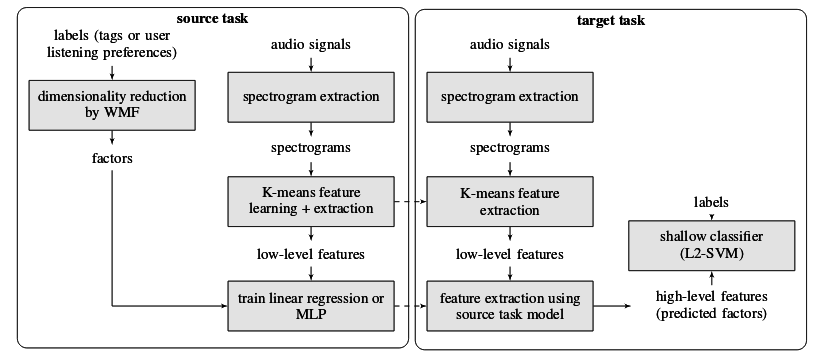
\includegraphics[width=0.95\textwidth]{specLeak1}
\caption{Schematic overview of the workflow of transfer learning}
 \label{fig:transfer learning}
 \end{figure}
\FloatBarrier
\bigskip

\noindent \textbf{Source task}: 
The low-level features from audio spectrograms are learned through unsupervised learning by spherical K-Means. To tackle problems created by redundant and sparse labels, dimensionality reduction is done in the label space using PCA. The model is then trained to predict the reduced label representation.
\bigskip

\noindent \textbf{Target task}
Next,  the trained models are used to extract higher-level features from other datasets, which are then passed to train shallow classifiers for different but related target tasks. This workflow is visualized in fig[ ] Dashed arrows indicate transfer of the learned feature extractors from the source task to the target task.
\bigskip

\noindent It has been shown that features learned in this fashion work well for auxiliary audio classification tasks on different datasets, consistently outperforming a purely unsupervised feature learning approach.

\subsection{Towards deep learning}
As alternative to the above systems, Deep Neural Networks(DNN) have recently become widely used in audio analysis, following their success in computer vision, speech recognition [19]. From an engineering perspective, DNNs sidestep the problem of creating or finding audio features relevant to a task. Their general structure includes multiple hidden layers with hidden units trained to represent some underlying structure in data.
